\documentclass[
]{article}

\usepackage{amsmath}

\usepackage{enumitem}
\setlistdepth{9}

\setlist[itemize,1]{label=\textbullet}
\setlist[itemize,2]{label=\textbullet}
\setlist[itemize,3]{label=\textbullet}
\setlist[itemize,4]{label=\textbullet}
\setlist[itemize,5]{label=\textbullet}
\setlist[itemize,6]{label=\textbullet}
\setlist[itemize,7]{label=\textbullet}
\setlist[itemize,8]{label=\textbullet}
\setlist[itemize,9]{label=\textbullet}

\renewlist{itemize}{itemize}{9}

\setlength\parindent{0pt}

\usepackage{ifthen}
\usepackage{trimspaces}

\usepackage{graphicx}
\usepackage{xesearch}
\usepackage[dvipsnames]{xcolor}
\makeatletter
\def\maxwidth{\ifdim\Gin@nat@width>\linewidth\linewidth\else\Gin@nat@width\fi}
\def\maxheight{\ifdim\Gin@nat@height>\textheight\textheight\else\Gin@nat@height\fi}
\makeatother
% Scale images if necessary, so that they will not overflow the page
% margins by default, and it is still possible to overwrite the defaults
% using explicit options in \includegraphics[width, height, ...]{}
\setkeys{Gin}{width=\maxwidth,height=\maxheight,keepaspectratio}
% Set default figure placement to htbp
\makeatletter
\def\fps@figure{htbp}
\makeatother

%\MakeBoundary{[}
%\UndoBoundary{]}

\UndoBoundary{[, ]}
\SearchList{startbrac}{}{*[?}
\SearchList{endbrac}{}{*]?}
%\SearchList{kbtag}{\color{ForestGreen}{\tiny\textulf{[[}\textbf{#1}\textulf{]]}}\color{black}}{*KB?}
\SearchList{kbtag}{\color{ForestGreen}{\href{http://taproot.shabang.cf/relay?request=#1}{\tiny\textulf{[[}\textbf{#1}\textulf{]]}}}\color{black}}{*KB?}




\providecommand{\tightlist}{%
  \setlength{\itemsep}{0pt}\setlength{\parskip}{0pt}}



\graphicspath{ {./} }

\usepackage{titlesec}
\usepackage{titling}
\usepackage{makecell}
\usepackage{bookmark}

\usepackage{float}
\let\origfigure\figure
\let\endorigfigure\endfigure
\renewenvironment{figure}[1][2] {
    \expandafter\origfigure\expandafter[H]
} {
    \endorigfigure
}

\usepackage{mathspec}
\setmainfont[
   ItalicFont     = HelveticaNeue-Italic,
   BoldFont       = HelveticaNeue-Bold,
   BoldItalicFont = HelveticaNeue-BoldItalic]{HelveticaNeue}
\newfontfamily\NHLight[
   ItalicFont     = HelveticaNeue-LightItalic,
   BoldFont       = HelveticaNeue-UltraLight,
   BoldItalicFont = HelveticaNeue-UltraLightItalic]{HelveticaNeue-Light}

\newcommand\textrmlf[1]{{\NHLight#1}}
\newcommand\textitlf[1]{{\NHLight\itshape#1}}
\let\textbflf\textrm
\newcommand\textulf[1]{{\NHLight\bfseries#1}}
\newcommand\textuitlf[1]{{\NHLight\bfseries\itshape#1}}

\usepackage[margin=1in]{geometry}

\usepackage{fancyhdr}
\usepackage{hyperref}

\usepackage{longtable,booktabs}
\usepackage{caption}
% Correct order of tables after \paragraph or \subparagraph
\usepackage{etoolbox}
\makeatletter
\patchcmd\longtable{\par}{\if@noskipsec\mbox{}\fi\par}{}{}
\makeatother
% Allow footnotes in longtable head/foot
\IfFileExists{footnotehyper.sty}{\usepackage{footnotehyper}}{\usepackage{footnote}}
\makesavenoteenv{longtable}


\newcommand{\thecourse}{ HIST201 }
\newcommand{\thelesson}{ Coloumb's Law }

\title{\textbf{\thecourse}\thelesson}

\pagestyle{fancy}

\fancyfoot{}

\makeatletter
\trim@spaces@in \thecourse
\trim@spaces@in \thelesson
\makeatother
\lhead{\textbf{\thecourse} \thelesson}
\rhead{\textrmlf{Compiled} \today}
\lfoot{Houjun Liu \(\cdot\) \textbf{2020-2021}}
\rfoot{\textrmlf{Page} \thepage}


\titleformat{\section}
{\Large}
{\textrmlf{\thesection} {|}}
{0.3em}
{\textbf}


\titleformat{\subsection}
{\large}
{}
{0em}
{\textbf}

\titleformat{\subsubsection}
{}
{}
{0em}
{\textbf}

\setlength{\parskip}{0.45em}

\newcounter{definitionct}
\newcommand{\definition}[3][]{
    \stepcounter{definitionct}
    \begin{center}
        Definition \arabic{definitionct} \(\cdot\) [ \textbf{#2} \textrmlf{#3} ]
        \ifthenelse{ \equal{#1}{} }
            {}
            {\\ \textrmlf{#1}}
    \end{center}
}

\begin{document}

% DID YOU SET SPELL????

\ifthenelse{ \equal{KB20200824163718}{} }
{}
{\textbf{Source}: \href{http://taproot.shabang.cf/relay?request=KB20200824163718}{\tiny\textulf{[[}\textbf{KB20200824163718}\textulf{]]}}}

\hypertarget{coulombs-law}{%
\section{Coulomb's Law}\label{coulombs-law}}

\begin{figure}
\centering
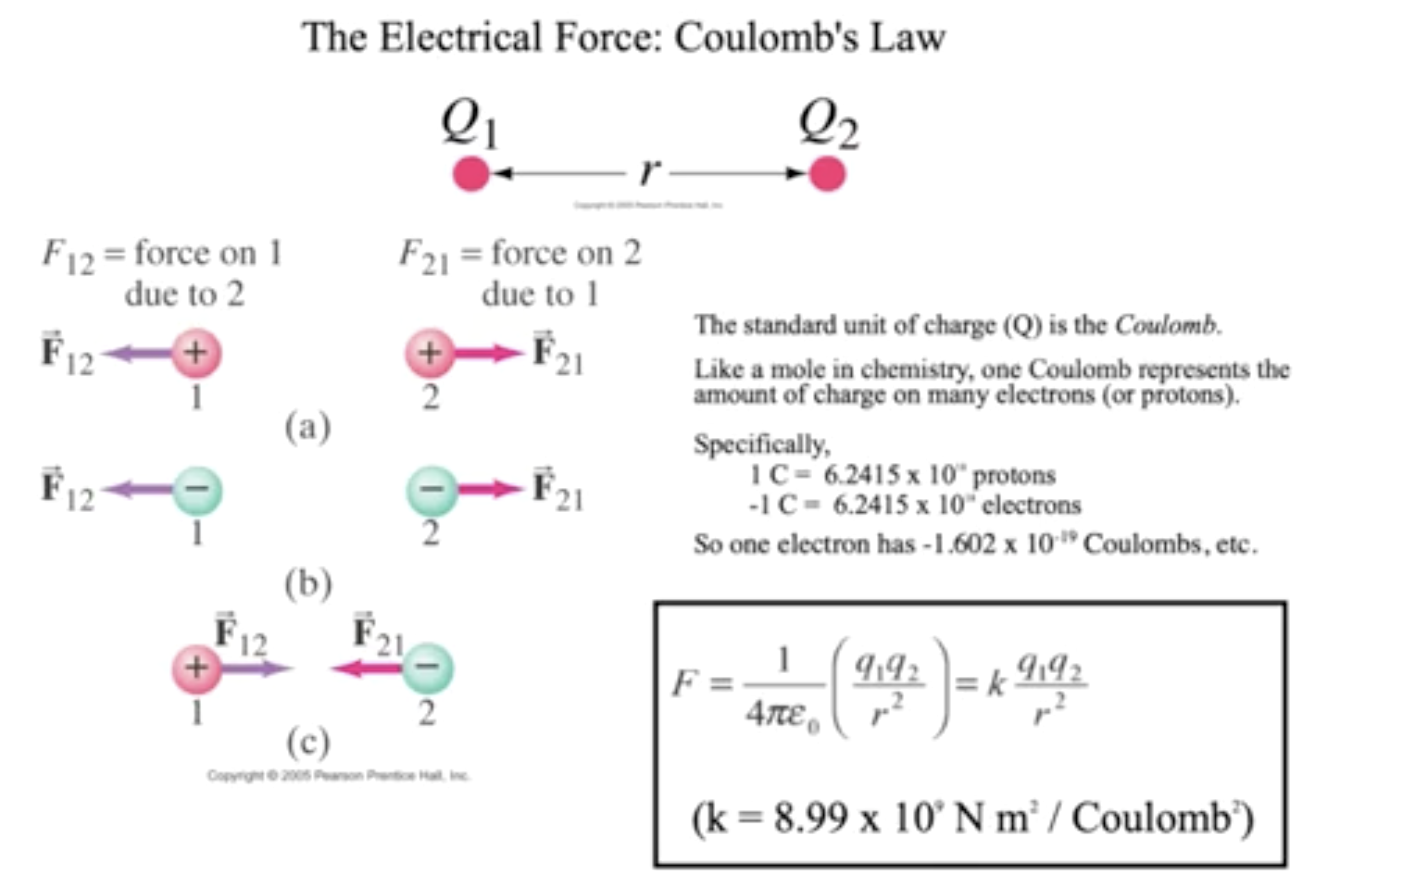
\includegraphics{/Users/houliu/Documents/School Work/2020-2021/KnowledgeBase/2020PHYS201/Screen Shot 2020-08-24 at 7.40.48 PM.png}
\caption{Screen Shot 2020-08-24 at 7.40.48 PM.png}
\end{figure}

\begin{itemize}
\tightlist
\item
  Electrical forces gets stronger as charge increases
\item
  Electrical forces gets weaker as charge decreases
\end{itemize}

\begin{quote}
The magnitude of force between two charges is given by the Columb's Law
\end{quote}

\definition[where $k$, a constant for change, $q_1$, change of first particle, $q_2$, change of second partical, $r^2$, distance squared]{Coulumb's Law}{$k\frac{q_1q_2}{r^2}$}

Note! The Standard Unit of Charge (Q) is the Coulomb --- a
representation for change for many electrons or many protons

\textbf{Remember this!}

\definition{Charge of an Electron}{$-1.602 \times 10^{-19} Q$}

\definition{k}{$8.99 \times 10^9 \frac{Nm^2}{Q^2}$}

\begin{quote}
E.M. forces, really, are two forces interacting with each other
\end{quote}

\textbf{Notice! Be careful with the signs when applying coulumbs law}

\begin{itemize}
\tightlist
\item
  If resulting Coulomb force \textgreater{} 0, force is REPULSIVE
  (became you multiplied positive to positive or negative negative)
\item
  If resulting Coulomb force \textless{} 0, force is ATTRACTIVE (became
  you multiplied positive to negative)
\end{itemize}

\hypertarget{guided-problem-solve}{%
\subsection{Guided Problem Solve}\label{guided-problem-solve}}

Special care must be taken for solving these problems w.r.t. to both
vector direction and multiple-atom-interactions
{[}{[}KB20200824224339{]}{]}

\hypertarget{heres-something-dna-replication}{%
\subsection{Here's something! DNA
Replication}\label{heres-something-dna-replication}}

\begin{figure}
\centering
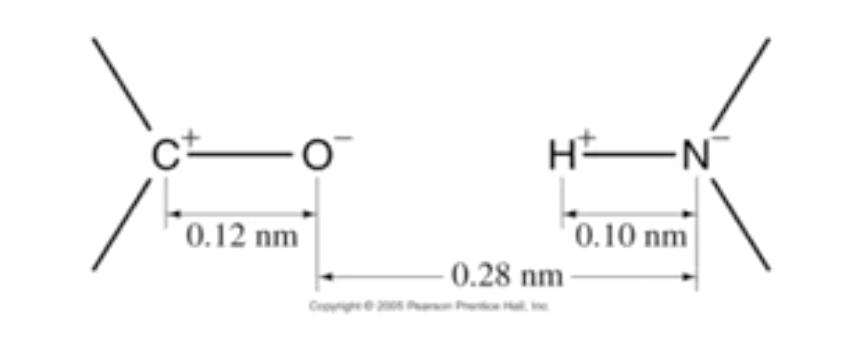
\includegraphics{/Users/houliu/Documents/School Work/2020-2021/KnowledgeBase/2020PHYS201/Screen Shot 2020-08-24 at 8.20.15 PM.png}
\caption{Screen Shot 2020-08-24 at 8.20.15 PM.png}
\end{figure}

The question is\ldots{} Between these four atoms, \emph{how many do we
need to calculate to find if these two repel or attract?}

This is fairly simple. Because of the fact every force between each pair
of atoms between these two elements needs to be calculated. So\ldots{} 2
(on the left) times 2 (on the right) = 4.

If these repel, the don't combine. If they attract, of course they do.

\end{document}
